\begin{figure}
\centering
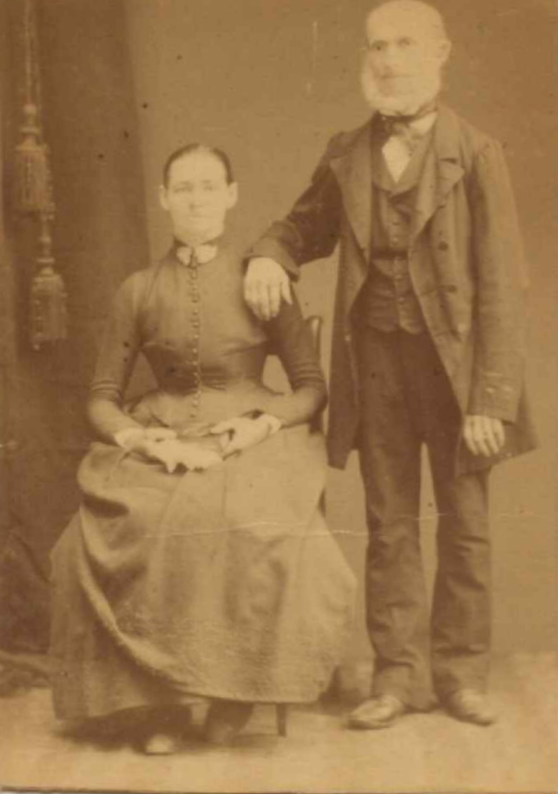
\includegraphics[width=\textwidth, height=\textheight, keepaspectratio]{222-a-frantisek_prusik-1823}
\caption{František Prusík, narozený 1823 v Nebřezinech, usazený v Plasích (1823 – 1902)}
\label{fig:222-a-frantisek_prusik-1823}
\end{figure}

             \begin{figure}
\centering
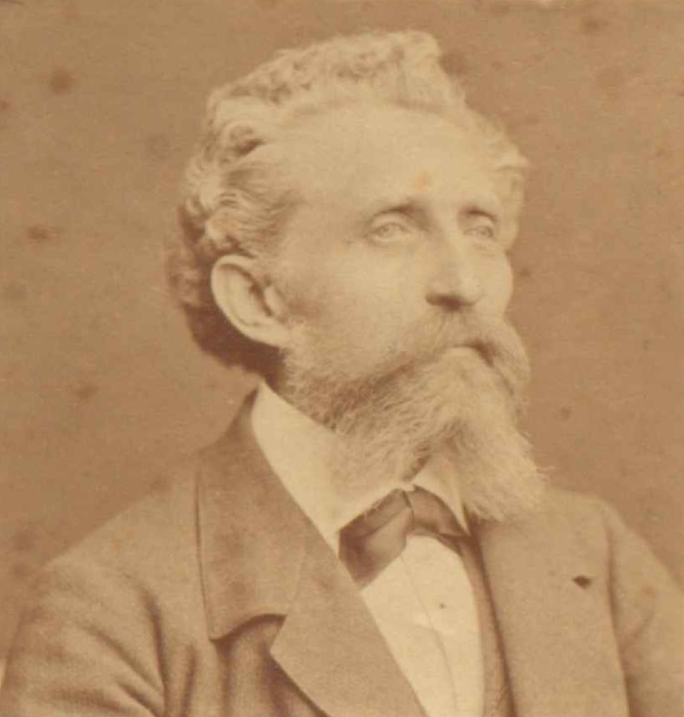
\includegraphics[width=\textwidth, height=\textheight, keepaspectratio]{222-b-josef_prusik_1826}
\caption{Josef Prusík, bratr Františkův, nar. 1826 v Nebřezinech a usazený v Praze (1826 – 1895)}
\label{fig:222-b-josef_prusik_1826}
\end{figure}

\begin{figure}
\centering
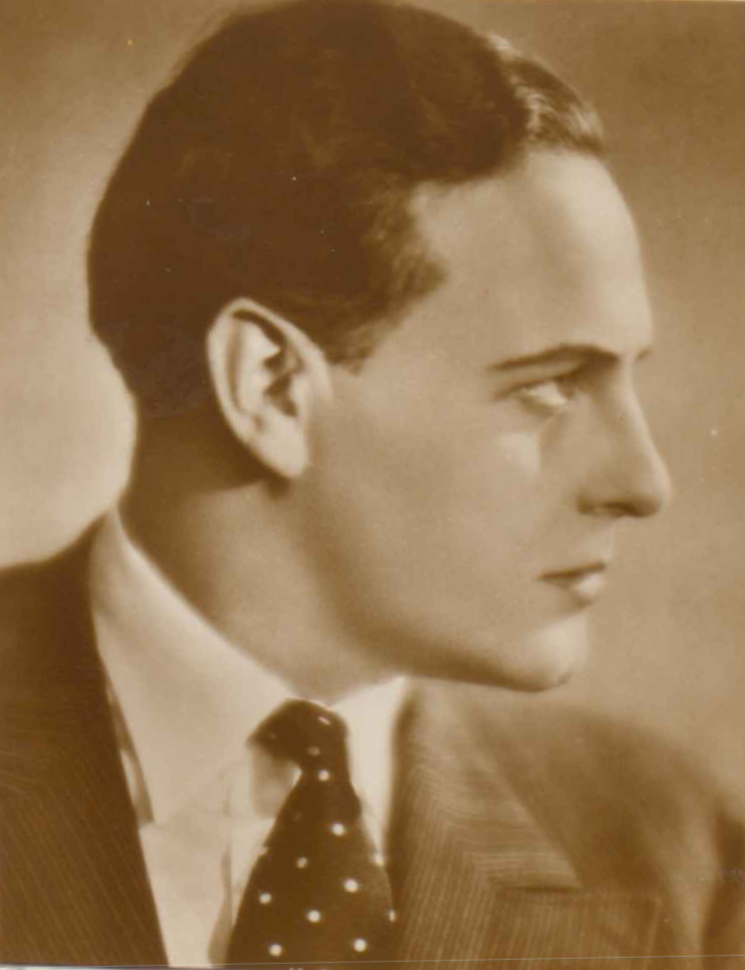
\includegraphics[width=\textwidth, height=\textheight, keepaspectratio]{222-c-karel_lamac}
\caption{Vnuk Josefa Prusíka Karel Lamač, průkopník českého filmu (1897 – 1952)}
\label{fig:222-c-karel_lamac}
\end{figure}


